\begin{donnees}
    \begin{itemize}
        \item $m=\qty{0.4}{\kg}$~; $\pi^{2}=10$~;
              les frottements sont négligeables.
    \end{itemize}
\end{donnees}
On écarte le solide $\mathrm{(S)}$ (Fig.~\ref{fig:solide_ressort}) de sa
position d'équilibre d'une distance $X_{m}$ et on le libère sans vitesse. On
repère la position du centre d'inertie $G$ par l'abscisse $x$ sur l'axe
$(O,\ex)$ et on choisit l'instant de passage de $G$ par la position d'équilibre,
avec la vitesse $v_{0}$, dans le sens positif comme origine des dates
$(t_{0}=0)$.


\begin{minipage}{0.64\linewidth}
    La courbe de la Fig.~\ref{fig:2bac_svt_national_2017_normale_phys_ex3_3}
    représente les variations de l'abscisse $x(t)$ du centre d'inertie $G$.
    \begin{enumerate}
    \item Déterminer graphiquement, les valeurs de la période propre $T_{0}$ et
          de l'amplitude $X_{m}$ du mouvement, puis trouver la valeur de $K$ (on
          prendra $\pi^{2}=10$).
    \item Calculer la valeur du travail de la force de rappel exercée sur ($S$)
          entre les instants $(t_{0}=0)$ et $(t_{1}=\frac{T_{0}}{4})$.
    \item En utilisant la conservation de l'énergie mécanique de l'oscillateur,
          déterminer la valeur de la vitesse $v_{0}$ à l'instant ($t_{0}=0$).
\end{enumerate}
\end{minipage}
\hfill
\begin{minipage}{0.34\linewidth}
\begin{figure}[H]
    \centering
    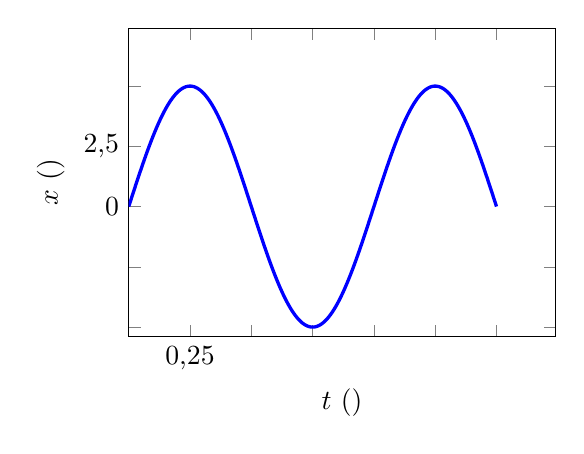
\begin{tikzpicture}
        \def\Xm{5}
        \def\T{1}
        \pgfmathpi\let\pi=\pgfmathresult
        \begin{axis}[
                xmin=0,xmax=1.74,
                ymin=-5.4,ymax=7.4,
                width=7cm,height=5.5cm,
                trig format plots=rad,
                xtick distance=0.25, ytick distance=2.5,
                xticklabels={,,{0,25}}, yticklabels={,,,0,{2,5}},
                xlabel=$t~(\unit{\second})$, ylabel=$x~(\unit{\cm})$,
                minor tick num=0,
            ]
            \addplot[domain=0:1.5,samples=200,very thick,blue]
                {\Xm*sin(2*pi/\T*x)};
        \end{axis}
    \end{tikzpicture}
    \caption{}
    \label{fig:2bac_svt_national_2017_normale_phys_ex3_3}
\end{figure}
\end{minipage}

